\documentclass[11pt, oneside]{article}   	% use "amsart" instead of "article" for AMSLaTeX format
\usepackage{geometry}                		% See geometry.pdf to learn the layout options. There are lots.
\geometry{letterpaper}                   		% ... or a4paper or a5paper or ... 
%\geometry{landscape}                		% Activate for rotated page geometry
\usepackage[parfill]{parskip}    		% Activate to begin paragraphs with an empty line rather than an indent
\usepackage{graphicx}				% Use pdf, png, jpg, or eps§ with pdflatex; use eps in DVI mode
								% TeX will automatically convert eps --> pdf in pdflatex		
\usepackage{amssymb}

\usepackage{pdfpages}
\usepackage{xcolor}
\pagecolor{white}
%SetFonts

%SetFonts


\title{ASTE 586 Computer Project Part 1}
\author{Andrew Gerth}
\date{19 February 2025}							% Activate to display a given date or no date

\begin{document}

\maketitle
%\section{}
%\subsection{}
\section{Introduction}
This report details the methodology and solution used to complete the ASTE 586 Spacecraft and Attitude Dynamics Computer Project (Part 1). 

The goal of this project was to numerically integrate a given initial value problem and compare the approximated solution to an exact analytical solution.

The initial value problem was given as a linear system of four Ordinary Differential Equations:


\[
\vec{\dot{x}}(t) = 
\left[
\begin{array}{ccc}
\dot{x_1}(t)\\
\dot{x_2}(t)\\
\dot{x_3}(t)\\
\dot{x_4}(t)
\end{array}
\right]
=
\left[
\begin{array}{cccc}
0 & 2 & 0 & 0 \\
-2 & 0 & 0 & 0 \\
0 & 0 & 0 & 200 \\
0 & 0 & -200 & 0
\end{array}
\right]
\left[
\begin{array}{ccc}
x_1(t)\\
x_2(t)\\
x_3(t)\\
x_4(t)
\end{array}
\right]
\]


The initial values were given as:

\[
\vec{x}(0) = 
\left[
\begin{array}{ccc}
x_1(0) \\
x_2(0) \\
x_3(0) \\
x_4(0)
\end{array}
\right]
=
\left[
\begin{array}{ccc}
1 \\
0 \\
1 \\
0
\end{array}
\right]
\]

The numerical and analytical solutions were to be compared to at least $t = 10$, ultimately achieving a maximum allowed difference of $10^-3$ or less for all four components of $x$.

The final demonstration to assess the accuracy of the numerical solution was to plot $x^2_1(t) + x^2_2(t) + x^2_3(t) + x^2_4(t) - 2$ versus time to demonstrate the result is very close to zero.



\section{Analytical Solution}
To solve the initial value problem, I recognized it was given in the form $\frac{d}{dt}\vec{x}(t) = [A]\vec{x}(0)$, which has a solution of $\vec{x}(t) = e^{At}\vec{x}(0)$.

To find $e^{At}$ I found the eigenvalues of $A$ by solving $det(A-\lambda I) = 0$ for $\lambda$. This resulted in 4 eigenvalues:



\[
\left[
\begin{array}{cccc}
\lambda_{1,2} \\
\lambda_{3,4}
\end{array}
\right]
=
\left[
\begin{array}{cccc}
\pm 2i \\
\pm 200i
\end{array}
\right]
\]

Next I solved $(A - \lambda_iI)\vec{v}_i = \vec{0}$  to find the eigenvectors corresponding to each eigenvalue.

\[
\left[
\begin{array}{cccc}
\vec{v}_1\\
\vec{v}_2\\
\vec{v}_3\\
\vec{v}_4
\end{array}
\right]
=
\left[
\begin{array}{cccc}
\left[1, i, 0, 0\right] \\
\left[1, -i, 0, 0\right] \\
\left[0, 0, 1, i\right] \\
\left[0, 0, 1, -i\right]
\end{array}
\right]
\]



Using the general solution of the form:\\
\[
\vec{x}(t) = c_1e^{\lambda_1t}\vec{v_1} + c_2e^{\lambda_2t}\vec{v_2} + c_3e^{\lambda_3t}\vec{v_3} + c_4e^{\lambda_4t}\vec{v_4}
\]

Next substitute the corresponding eigenvectors and eigenvalues:\\

\[
\vec{x}(t) = c_1e^{2it}
\left[
\begin{array}{ccc}
1 \\ i \\ 0 \\ 0
\end{array}
\right]
+ c_2e^{-2it}
\left[
\begin{array}{ccc}
1 \\ -i \\ 0 \\ 0
\end{array}
\right]
+ c_3e^{200it}
\left[
\begin{array}{ccc}
0 \\ 0 \\ 1 \\ i
\end{array}
\right]
+ c_4e^{-200it}
\left[
\begin{array}{ccc}
0 \\ 0 \\ 1 \\ -i
\end{array}
\right]
\]



\[
\vec{x}(t) = 
\left[
\begin{array}{ccc}
c_1e^{2it} + c_2e^{-2it}\\
ic_1e^{2it} - ic_2e^{-2it}\\
c_3e^{200it} + c_4e^{-200it}\\
ic_3e^{200it} - ic_2e^{-200it}\\
\end{array}
\right]
\]


Use Euler's Formula: \\
\[
e^{i\omega t} = cos(\omega t) + isin(\omega t)
\]
\[
\vec{x}(t) = 
\left[
\begin{array}{ccc}
 A_1cos(2t) + A_2sin(2t) \\ 
 -A_1sin(2t) + A_2cos(2t) \\
 A_3cos(200t) + A_4sin(200t) \\
-A_3sin(200t) + A_4cos(200t)
\end{array}
\right]
\]

	where\\

\[
\vec{A} = 
\left[
\begin{array}{ccc}
c_1 + c_2 \\
 i(c_1 - c_2)\\
 c_3 + c_4\\
 i(c_3 - c_4)\\
\end{array}
\right]
\]



Now to solve for the coefficient vector $\vec{A}$, evaluate at the initial condition $t = 0$.

$\vec{A} = [1, 0, 1, 0]$

This gives the analytical solution to the linear system of equations:



\[
\vec{x}(t) = 
\left[
\begin{array}{ccc}
 cos(2t)  \\
 -sin(2t)  \\
 cos(200t)  \\
 -sin(200t)
\end{array}
\right]
\]


\section{Numerical Integration}
My numerical integrations strategy was to use an already-built method of the Python library \verb!scipy!. This allowed me to minimize scripting, debugging, and testing time. 

The \verb!scipy.integrate.solve_ivp()! function allows for many different numerical integration methods and tolerances to be used. I chose the Runge-Kutta45 method and specified desired relative and absolute tolerances of $10^{-8}$. This combination ensured the solver met the specified accuracy from the problem statement while not being too computationally expensive.

\section{Plotting and Comparing Results}
Due to the linear system containing different orders of effects $x_1$ and $x_2$ on different order of magnitude than $x_3$ and $x_4$, I chose to create two sets of plots with different "step sizes" for clarity.
Figure 1 shows four plots.
\begin{enumerate}
\item Analytical Solution evaluated from $t = [0, 10]$ with step size of $0.100$.
\item Numerical Solution evaluated from $t = [0, 10]$ with step size of $0.100$.
\item Absolute Error (defined as $x_{analytical}(t) - x_{numerical}(t)$) for the same range and step size.
\item The result of $x^2_1(t) + x^2_2(t) + x^2_3(t) + x^2_4(t) - 2$ for the same range and step size.
\end{enumerate}

Figure 1 shows that the numerical solution is within the tolerances specified in the problem statement, but it does not show an accurate representation for the $x_3$ and $x_4$ terms due to the relatively large step size.

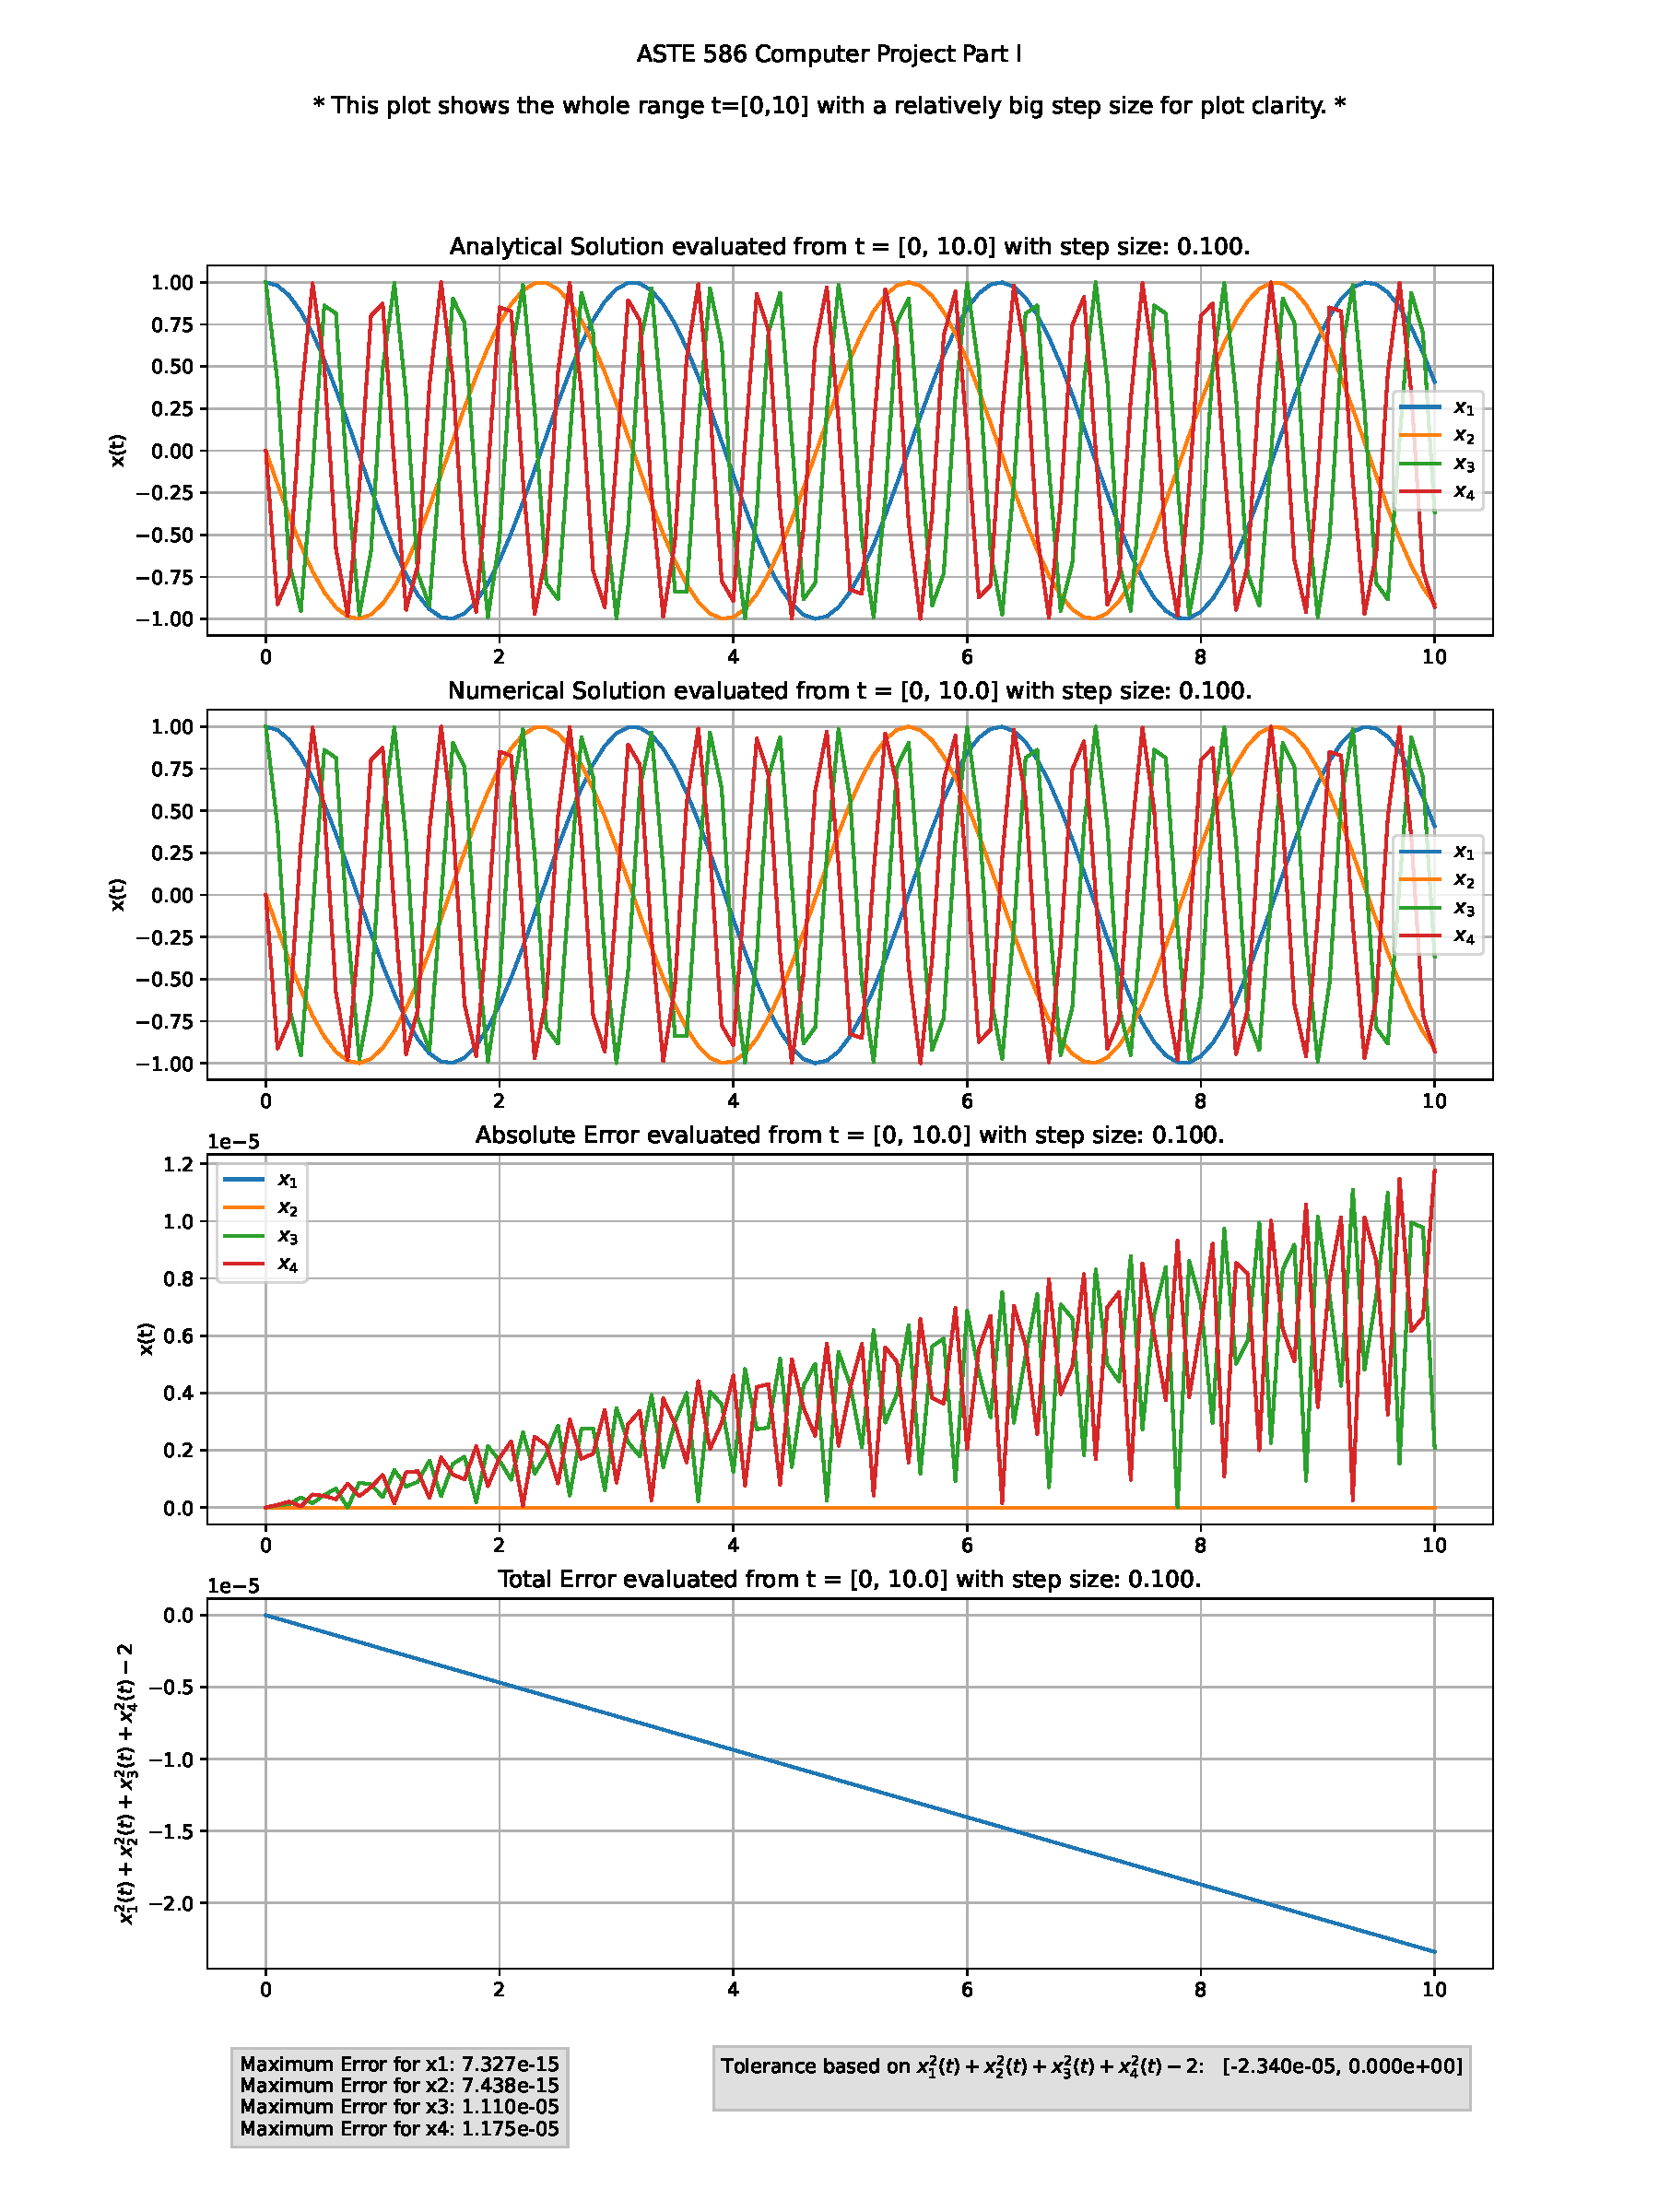
\includepdf[pages=-]{ASTE586_ComputerProject_Part1_Plot1.pdf}

Figure 2 contains the same set of four plots, but evaluated from $t = [0, 10]$ with step size of $0.00001$. The plots are then only shown from $t = [9.9, 10.0]$ as this is the most interesting region due to the highest amount of propagation error. 

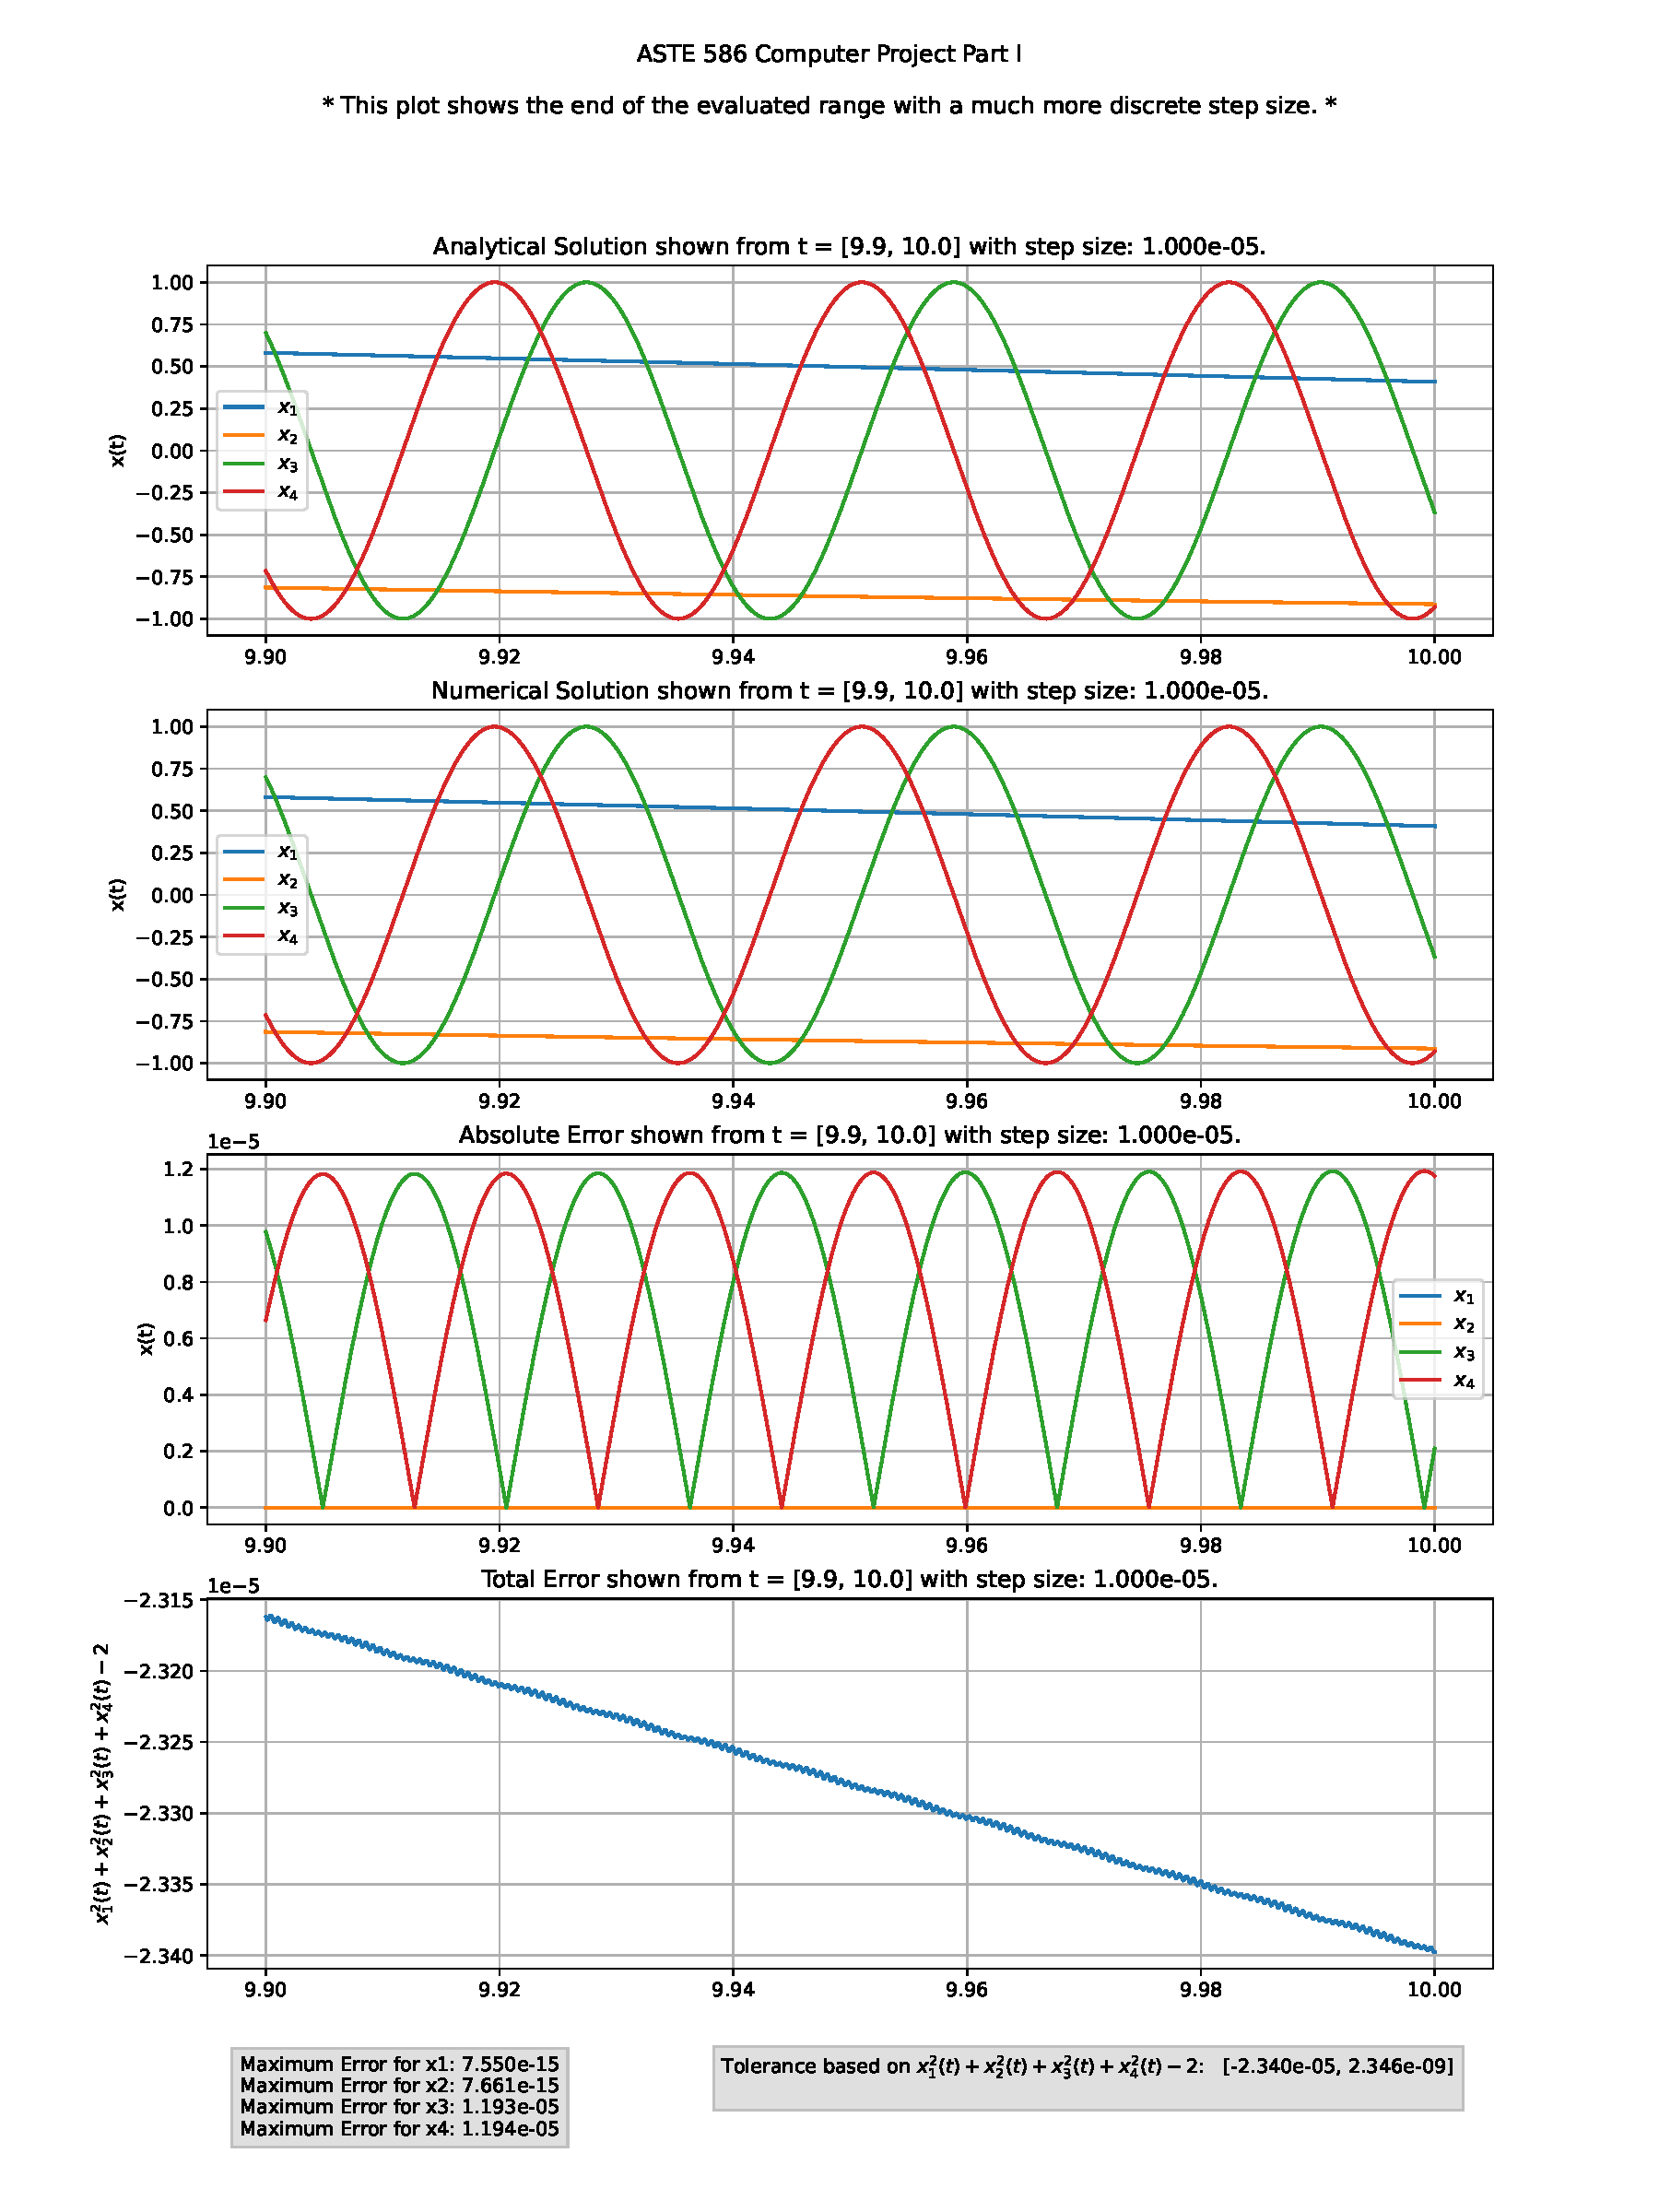
\includepdf[pages=-]{ASTE586_ComputerProject_Part1_Plot2.pdf}
%![[ASTE586_ComputerProject_Part1_Plot2.pdf]]

These four plots show the behavior of $x_3$ and $x_4$ much more accurately and serve as a good final confirmation that the goal of the computer project has been satisfied.

The maximum absolute error (*note all maximum errors do not occur at the same value of $t$):

$x_1: 7.550\times10^{-15}$\\
$x_2: 7.661\times10^{-15}$\\
$x_3: 1.193\times10^{-05}$\\
$x_4: 1.194\times10^{-05}$

The tolerance based on $x^2_1(t) + x^2_2(t) + x^2_3(t) + x^2_4(t) - 2$ was: 

$[-2.340\times10^{-05}, \space \space 2.346\times10^{-09}]$

\section{Conclusion}
The initial value problem was solved analytically and numerically. The accuracy of the numerical solver met the requirements and is also easily tuned for different required accuracies within the method. For further details on the solver script and the analytical derivation, please see the attachments to this report.


\section{Appendix A: Python Script}
See following page.
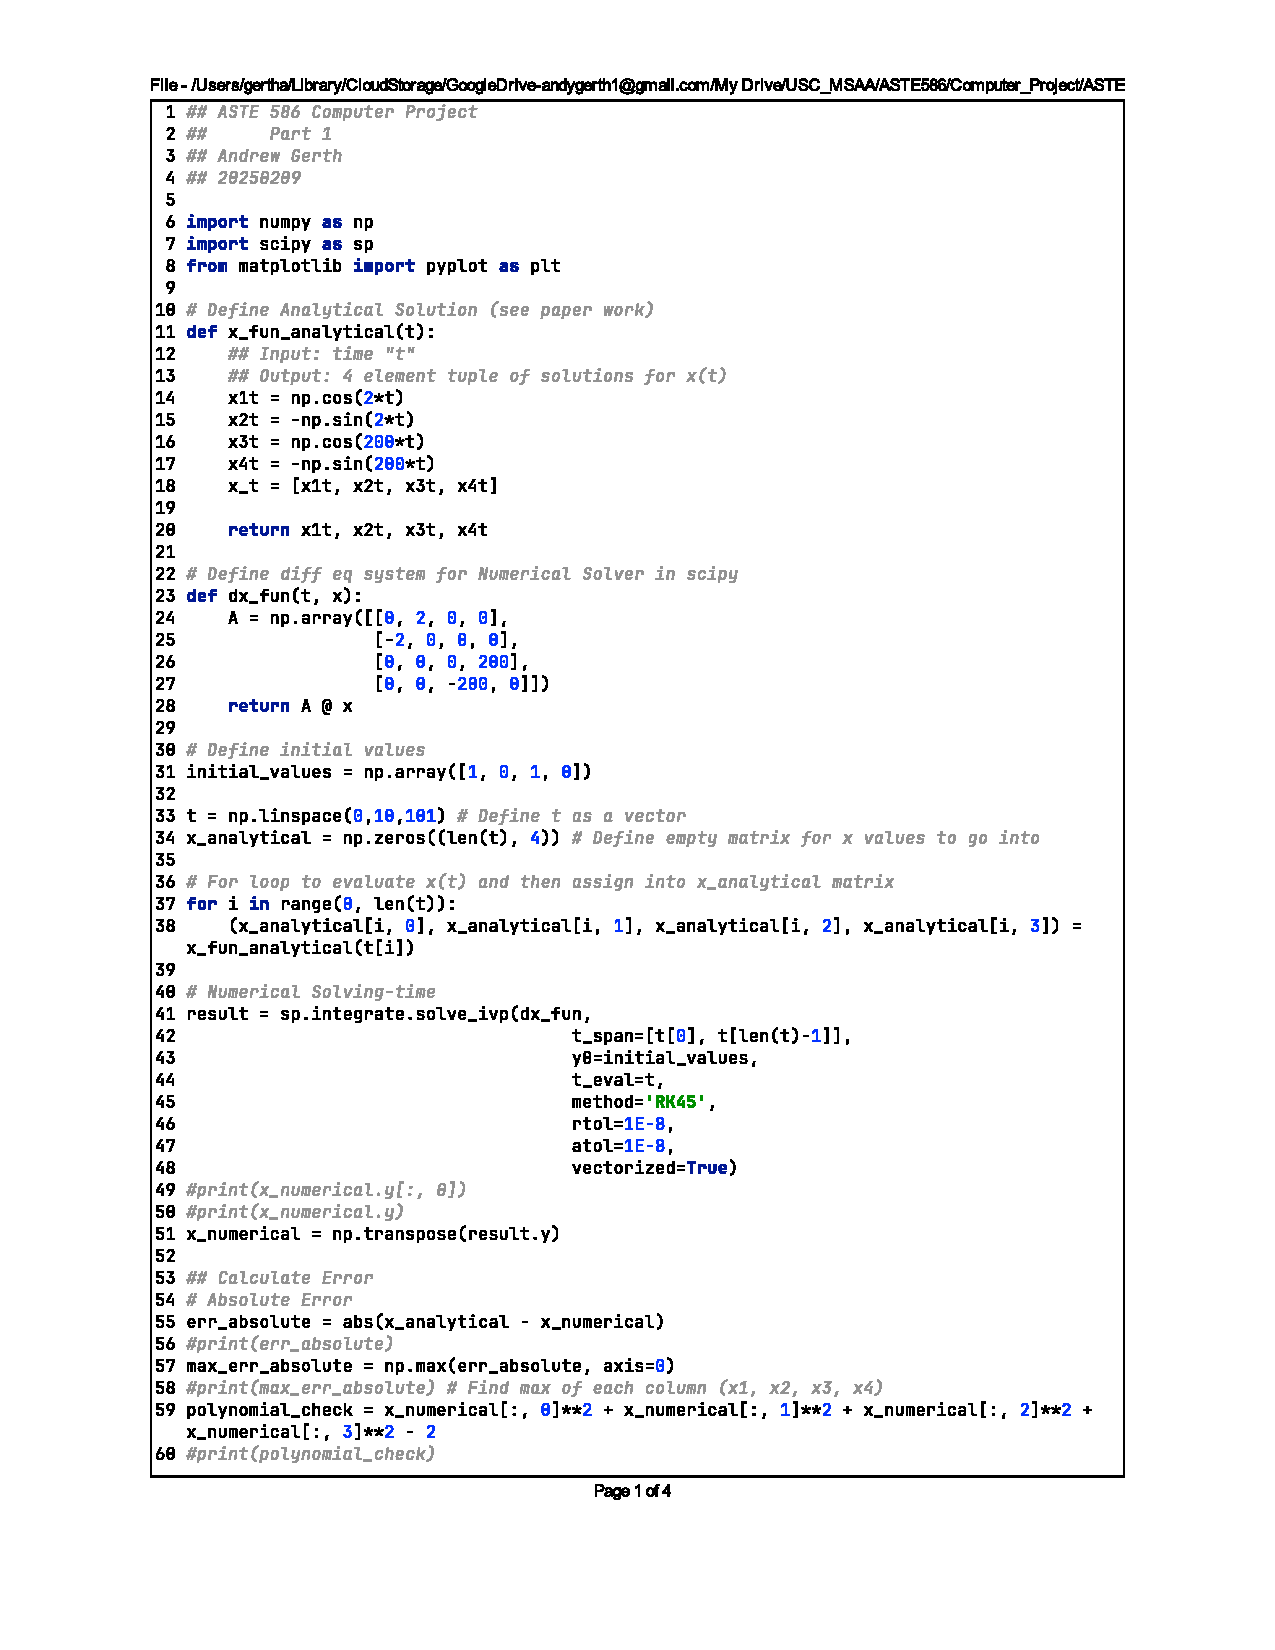
\includepdf[pages=-]{ASTE86_ComputerProject_Part1_Code_GerthAndrew.pdf}


\section{Appendix B:  Detailed Derivation of Analytical Solution}
See following page.

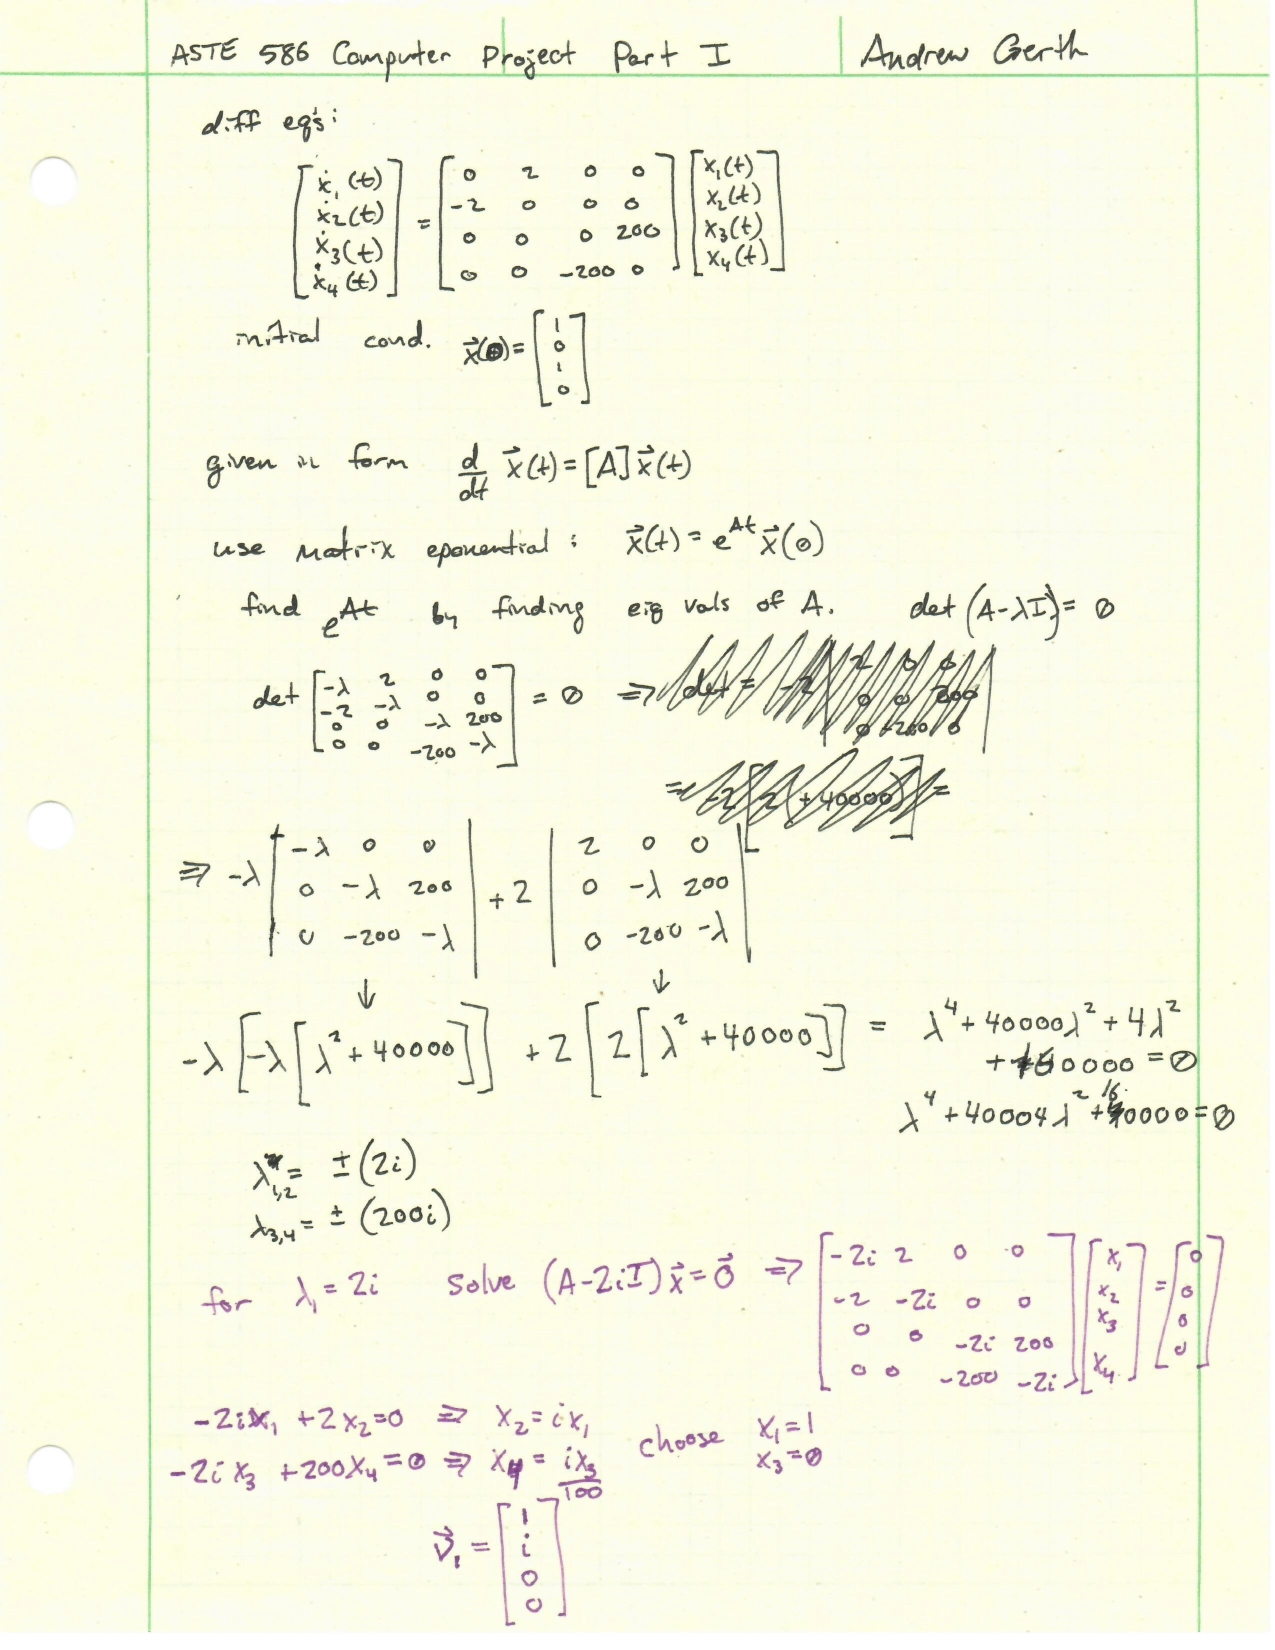
\includepdf[pages=-]{ASTE586_ComputerProjectPart1_GerthAndrew_paper.pdf}



\end{document}  
